%===================================================================================================
%  Chapter : ベクトル解析
%  説明    : ベクトル解析について説明する.
%===================================================================================================
%   %==========================================================================
%   %  Section
%   %==========================================================================
 \section{ベクトル関数}
    \subsection{ベクトル変数(あるいは,変数ベクトル)}
    ベクトルには,スカラーにおける語彙「変数」に対応する,一般的呼称がない.
    ないと不便なので,このノートでは \textbf{ベクトル変数} という言い方を導入する.
    もしかしたら,\textbf{変数ベクトル} と書くこともあるかもしれない.

    細かいことを言うと,ベクトル変数は,
    成分の一部あるは全部が変数であるようなベクトルであり,
    次に説明するベクトル関数である
        \footnote{
            定義が論理的に循環してしまっているが,意図は伝わるはず.
            循環しないような記述も可能だが,理論構築が目的ではない
            ため,深く突っ込まないでおこう.
        }.

    変数をベクトル変数と区別する意味で,\textbf{スカラー変数} と
    書くこともある.

    \subsection{ベクトル関数}
    ベクトルが絡む関数のことを総称して \textbf{ベクトル関数} という.
    また,ベクトル関数と区別するために,
    今まで考えてきたベクトルが絡まないような関数を,
    \textbf{スカラー関数} と表現する場合がある
        \footnote{
            細かいことを言うと,スカラーは1次元ベクトルだから,
            スカラー関数もベクトル関数である.
        }.

    考えれる例をいくつか上げておこう.特にこれらを区別してよぶ必要は
    ないので,名称を与えることはしない
        \footnote{
            記述の際には,どんな形の
            ベクトル関数について議論している
            かが明確にわかるようにする.
        }.

    例えば,スカラーの独立変数 $t$ に対して,
    1つの定ベクトルが定まる関数が考えられる.これを
        \begin{align}
            \ba (t)
        \end{align}
    と表す.
    関数記号 $\ba$ を太字にした意図は,
    ベクトルが定まる(値域がベクトルである)ことを明示するためである.
    また,$(t)$ という表記は,$t$ が独立変数であることを示すものである
        \footnote{
            多変数になる場合,$\ba(t,\,s)$ と書かれることになる
            ($t$ と $s$ はスカラーである).
            このとき,$(t,\,s)$ という記述がベクトルを成分表示と同じで,
            紛らわしいかもしれない.しかし,文脈により容易に区別できる
            とし,特に書き分けることはしない.この記述の前に関数を
            表現する文字があれば,それらは独立変数である.
        }.

    別の例を上げると,ベクトル変数を独立変数にもつ関数が考えられる.
    数式で表そうとすると,
        \begin{align}
            \ba (\br)
        \end{align}
    のようになる.$\br$ はベクトル変数である.

    上記2つの混合して,スカラー変数 $t$ とベクトル変数 $\br$ から
        \begin{align}
            \ba (t,\,\br)
        \end{align}
    という関数を作ってもいい.

    ベクトル変数を独立変数として,スカラーが定まる(値域がスカラーである)
    関数もあり得る.記号化すれば,
        \begin{align}
            a (\br)
        \end{align}
    となるだろう.関数記号 $a$ を細字にした意図は,スカラーが定まることを
    明示するためである.

    もちろん,スカラー変数 $t$ とベクトル変数 $\br$ をもち,
    スカラーが定まる関数も考えられる.
        \begin{align}
            a (t,\,\br)
        \end{align}

    定ベクトルもベクトル関数の一部として考える.
    明示的な独立変数はないが,入力にかかわらず常に一定値をとるような
    関数として捉える.スカラー関数の場合と同じように考える.

    独立変数が1つのベクトル関数($\ba(t)$)を,\textbf{1変数ベクトル関数} という.
    独立変数が2つ以上のベクトル関数を総称して,\textbf{多変数ベクトル関数} という.
    ベクトル変数をもつベクトル関数($\ba(\br)$ など)は多変数ベクトル関数として考える.

    ひと目で見やすいように,表にしておこう(\Table\ref{table:f4unit}).
        \begin{table}[htb]
          \centering
          \caption{ベクトル関数の種類}
          \begin{tabular}{|l|c|c|l|}                                        \hline
            関数記号      & 独立変数   & 値域     & 例                      \\ \hline  \hline
            $\ba$         & なし       & ベクトル & 定ベクトル              \\ \hline
            $\ba(t)$      & $t$        & ベクトル & ある1点の風向の時間推移 \\ \hline
            $\ba(\br)$    & $\br$      & ベクトル & ある時刻の風向分布      \\ \hline
            $\ba(t, \br)$ & $t$,$\br$ & ベクトル & 風向分布の時間推移      \\ \hline
            $a(\br)$      & $\br$      & スカラー & 風力分布                \\ \hline
            $a(t, \br)$   & $t$,$\br$ & スカラー & 風力分布の時間推移      \\ \hline
          \end{tabular}
          \label{table:f4unit}
        \end{table}

    \subsection{ベクトル関数の微積分}
    \begin{mycomment}
        スカラー関数での微積分を,ベクトル関数へ拡張する.
        ベクトル関数の微積分も,基本的にはスカラー関数と同じように
        計算可能である.
    \end{mycomment}

    \subsubsection{極限}
    ベクトル関数の極限はスカラー関数の場合と同じように定義できる.

    \subsubsection{導関数}

 \subsection{使用用語}
    電磁気学を考えるとき,\textbf{曲線} や,\textbf{閉曲線} 等という数学用語を
    頻繁に使う.ニュートン力学では,特に必要はない
        \footnote{
            知っていれば,それだけ“広く”考えられるが,
            無理してまで,ここで学習する必要はない.
        }.
    だから,電磁気学を学習し始める段階になったら,この部分を読むようにすればいい.

    最初に,これらの用語について,あらかじめ
    確認する.以下の説明はすごく感覚的なものであって,
    全く厳密でないことを注意しておく.

 \subsubsection{導線(曲線)}
    一本のひものように,端と端が結ばれていない線のことを 曲線 という.
    このノートでは,「電気の流れる道」という意味をこめて,\textbf{導線} と
    いうことにする.導線の形は グニャグニャ と曲がっていてかまわないが,
    導線が自身と重ならないようなものであるとする(リボンのように絡まっていないものする).
    このノートでは,導線を表現する記号として,$\Gamma$ を用いる.
                \begin{figure}[hbt]
                    \begin{center}
                        \includegraphicslarge{kyokusenn.pdf}
                        \caption{導線}
                        \label{fig:kyokusenn}
                    \end{center}
                \end{figure}

    数学的に表現すると,曲線とは各成分が共通のパラメータ $t$ の
    関数であるようなベクトルのことをいう.式で表せば,曲線 $\br(t)$ は
        \begin{align}
            \br_{n}(t)=\left( x_{1}(t),\,x_{2}(t),\,x_{3}(t),\cdots ,\,x_{n}(t)\right)
        \end{align}
    と書ける.これは $n$ 次元ベクトルである.
    このノートでは空間の次元である3次元を考えているので,その各成分は $\left(x(t),\,y(t),\,z(t)\right)$ と書くことにし,
        \begin{align}
            \br(t)=\left( x(t),\,y(t),\,z(t)\right)
        \end{align}
    とする.この式は時刻 $t$ における位置を表現する式と同じである.時間 $t$ を正方向に
    なめらかに変化させていき,その各々の時間における位置を記録していけば,1つの曲線が現れてくる.
    力学ではこの曲線のことを「軌跡」とよんでいたが,ここではそれを一般的に解釈して,\textbf{曲線} と
    いうことにする.このノートの電磁気学の部分においては,曲線として出てくるのは回路の導線である.そこで,曲線とよばずに,
    \textbf{導線} ということが多い.また,導線の形をいちいち指定することはしない.だから,$\Gamma=\br(t)$ として,
    導線を表現する記号として,$\Gamma$ を用いる.

    以下では導線は連続しているという条件を課する.簡単にいえば,「切れていない」導線を考えるということである.

 \subsubsection{閉曲線}
    導線の両端がつながっているとき
    \footnote{
        この場合,どこが端であるかは見分けがつかないが….
    }
    ,これを \textbf{閉曲線} という.
    閉曲線の形は    グニャグニャ と曲がっていてもよいが,
    「八の字」のように導線同士が接触してが重ならないようにする.
    輪ゴムのようなものを考えるとよい.
    このノートでは,閉曲線を表現する記号として,$l$ を用いる.

                \begin{figure}[hbt]
                    \begin{center}
                        \includegraphicsdefault{heikyokusenn.pdf}
                        \caption{閉曲線}
                        \label{fig:heikyokusenn}
                    \end{center}
                \end{figure}

 \subsubsection{曲面}
    平らではなく,  グニャグニャ とした面のことを \textbf{曲面} という.
    もちろん,平らな面も曲面に属するが,ここではもっと一般的なグニャッと
    なった面を想像してもらいたい.

    電磁気学では特に,「縁をもった曲面」を考えることも多い
        \footnote{
        例えば,お皿等がその例になるだろう.
        縁を持たない曲面の例とは,ボールの表面があげられよう.
        }.
    曲面の境界は
    閉曲線である.従って以下では,「縁をもった曲面」のことを
    『閉曲線 $l$ を縁とする曲面』
    のようにいうことにする.
    このノートでは,閉曲線 $l$ を縁とする曲面 を 表現する記号として,
    $S_{l}$ を用いることにする.

 \subsubsection{閉曲面}
    ボールの表面のように,縁をもたない曲面のことを \textbf{閉曲面} という.
    グニャグニャとしていてよいが,面同士が重なったり,互いに切断しあったりしない
    ものとする.    このノートでは,閉曲面を表現する記号として,$S$ を用いる.

    ここで
    注意したい,「閉曲線 $l$ を縁とする閉曲面 $S_{l}$」と「閉曲線 $S$」の違いである.
    $S$ の添え字に $l$ が付いているもの($S_{l}$)は曲面であり,
    添え字に $l$ がついていないもの($S$)は閉曲面である.
                \begin{figure}[hbt]
                    \begin{tabular}{cc}
                        \begin{minipage}{0.5\hsize}
                    \begin{center}
                        \includegraphicsdouble{kyokumenn.pdf}
                        \caption{曲面}
                        \label{fig:kyokumenn}
                    \end{center}
                        \end{minipage}
                        \begin{minipage}{0.5\hsize}
                    \begin{center}
                        \includegraphicsdouble{heikyokumenn.pdf}
                        \caption{閉曲面}
                        \label{fig:heikyokumenn}
                    \end{center}
                        \end{minipage}
                    \end{tabular}
                \end{figure}

 \subsubsection{領域}
    閉曲面 $S$ を考えるとき,その表面は その内側の空間 と 外側の空間 を分けていると
    考えられる.閉曲面の内側の空間のことを \textbf{領域} という.
    領域を表現する記号として,このノートでは $\Omega_{S}$ を用いる.もちろん,
    添え字の $S$ は領域の表面である閉曲面 $S$ を意味している.
                \begin{figure}[hbt]
                    \begin{center}
                        \includegraphicsdefault{ryouiki.pdf}
                        \caption{領域}
                        \label{fig:ryoiki}
                    \end{center}
                \end{figure}

 \subsection{線積分と面積分のイメージ}
    \begin{quotation}\small
    線積分と面積分についての詳しいことは,
    ベクトル解析の教科書や微分積分学の教科書
    を参照してもらうことにして,ここではそのイメージを
    記述しておく.
    \end{quotation}

 \subsection{ベクトル空間}
    位置を一つ指定すると,その位置に対して,
    1つのベクトルが指定される空間を考える(図\ref{fig:vector_sp}参照).
                \begin{figure}[hbt]
                    \begin{tabular}{cc}
                        \begin{minipage}{0.5\hsize}
                            \begin{center}
                                \includegraphicslarge{vector_sp.pdf}
                                \caption{ベクトル空間1(説明図)}
                                \label{fig:vector_sp}
                            \end{center}
                        \end{minipage}
                        \begin{minipage}{0.5\hsize}
                                \begin{center}
                                \includegraphicslarge{vector_sp2.pdf}
                                \caption{ベクトル空間2(イメージ)}
                                \label{fig:vector_sp2}
                            \end{center}
                        \end{minipage}
                    \end{tabular}
                \end{figure}

    任意の位置 $\br$ に対して,
    1つのベクトル $\bA$ が
    決定されるという空間をイメージして描いた図である.
    このような空間を \textbf{ベクトル空間} という.
    また,位置(と時間)を指定すると
    1つのベクトルを決定できるので,
    これは関数の性質に他ならず,
    これを \textbf{ベクトル関数} という.
    従って,$\bA$ を $\bA(\br)$ と
    表現したほうがベクトル関数であることが,明確になる.
    しかし今後も,式が煩雑にならないように,
    ベクトル関数の変数である $\br$ を
    省略して表現する($\bA:=\bA(\br)$).

    ベクトル空間の例としてよく取り上げられる現象のうち,
    空気の流れ(風)がある.風は向きと速度をもっている.
    その向きと速度は場所と時間によって異なるが,
    1つの場所と時間を指定すれば,風の向きと速度は
    求まる.
    川の流れや,海水の流れといった現象も
    ベクトル空間で表現される.要するに,
    何かの「流れ」があったときに,
    それはベクトル空間で表現するのである.

    以下でベクトル空間というときには,図\ref{fig:vector_sp2}
    を思い浮かべてもらいたい.但し,
    ベクトル $\bA$ については,
    時間と位置を指定すれば決定されるようなものであれば,
    図\ref{fig:vector_sp2}のようなものでなくとも,自由に想像してよい.



 \subsection{ベクトルとスカラーの区別の仕方}
                いままで,ベクトルとは大きさと向きのある量であると
                考えてきた.また,スカラーは大きさのみをもつ量とし
                ていた.実は,これは正確な説明ではない.ベクトル空間を
                確認した今,ベクトルとスカラーの正確に違いについて,
                議論ができる.ここで整理しよう.

                ベクトルとスカラーを正確に区別する方法は,座標変換を
                考えることである.私がある空間に直交座標を張ったとしよう.
                私のいる空間には,複数の人がいて,その各々が任意に
                直交座標を張るとする.もちろん,何人もの人が張った直交
                座標の座標軸の方向はばらばらである.

                この空間が,ベクトル空間であったとしよう.その時,私は
                1つの点に属する1つのベクトルをみるとする.
                そのベクトルの方向は,私から見た方向と,他の観測者から見た
                方向とで一致しない
                    \footnote{
                        偶然の一致は起こりえるが,より一般的に考えよう.
                    }.
                それでは,この空間がベクトル空間ではなく,スカラー空間であるとしよう.
                この時には私がさしている点に属する数は,別の観測者が
                それを見ても,全く一致する.ベクトルとスカラーの違いは
                ここにある.私が見るベクトルの向きと,他の人が同じベクトルを見たときの
                むきは異なるが,スカラーは度の観測者に対しても同じ値を示す.
                観測者によって違うということは,直交座標の座標軸の設定方向が違う
                ということである.つまり,別の座標に移ってしまうと,ベクトルの向きは
                変化してしまうのである.スカラーは座標が変わっても,全く同じように
                観測される.両者はこのように,座標変換によって区別されるものである.
                座標変換についての知識がないので,これ以上ここでは話を続けることができない.
                座標変換について学ぶときに,もう一度,
                ベクトルとスカラーの違いを確認し,“実感”したいと思う.ここでは
                区別の仕方が知識として身に付いていれば,それでよいことにしよう.


 \subsection{線積分}
    ベクトル空間に,任意の曲線 $C$ を描く.
    この曲線 $C$ 上の全ての点にはそれぞれ1つの
    ベクトルが対応している.ベクトル空間に
    曲線 $C$ を描いてみると図\ref{fig:sensekibun}のようになる.
                \begin{figure}[hbt]
                    \begin{center}
                        \includegraphicslarge{sensekibun.pdf}
                        \caption{線積分}
                        \label{fig:sensekibun}
                    \end{center}
                \end{figure}


    見易さのために,曲線 $C$ 上のベクトルしか描いていないが,
    実際は別の点においてもベクトルは存在している.
    線積分の考察の対象はあくまでも,曲線 $C$ 上のベクトルだけである.

    曲線 $C$ を微小な長さの直線分割して,そのひとつひとつを $\df l$ とする.
    この部分の単位接線ベクトルを $\bt$ で表現する.
    もちろん,曲線 $C$ は曲がっているので,各 $\df l$ 部分における
    単位接線ベクトル $\bt$ は一定ではない.
    これらにより,長さ $\df l$ で向きが $\bt$ である
    ベクトル $\bt\,\df l$ を曲線 $C$ 上に
    作ることができる.$C$ 上に位置するベクトル $\bA$ の
    接線方向は  $\bA\cdot\bt\,\df l$ と
    表現できる.これを曲線 $C$ 全域にわたって積分したものが,
    線積分であり,
        \begin{align}
        \int_{C} \bA\cdot \bt\df l
        \end{align}
    と表現される.

    曲線 $C$ 上のベクトル $\bA$ の曲線方向成分 $\bt$ の
    積分を表している.


    \begin{memo}{詳細}
        もう少し優しく解説してみる.線積分とは,曲線 $C$ 上のベクトル関数を
        ,曲線 $C$ に沿って積分するということである.
        「曲線 $C$ に沿って積分する」というのは,ベクトル関数の曲線方向成分の
        総和を考えるということである.そのためには,曲線 $C$ とその上のベクトル $\bA$ の
        内積を考える必要がある
        \footnote{
        任意の2つのベクトル $\textit{\textbf{u}}$,$\bv$ の
        内積は $\textit{\textbf{u}}\cdot\bv=uv\cos\theta$ である.
        }
        すなわち,曲線をベクトルとしてみることが要求され,曲線に向きをつけるということである.
        曲線の向きは2通り考えられるが
        \footnote{
        曲線の両端をそれぞれA,Bとして,まず第1にAからBに向かう向きを考えられる.
        また,第2に,BからAに向かう向きを考えられる.
        }
        ,どちらをとろうが,結果は同じである.しかし,一度向きを指定したら,
        後になって変更することはできない.

        曲線 $C$ を有限の $N$ 個に分割しする(\ref{fig:senseki2}参照).
        このように分割された曲線は,ほとんど直線と見ることができる.
        つまり,曲線 $C$ を $N$ 個の直線で近似するのである.
        これらの近似的直線に名前と番号をつけて $\Delta l_{1}$,$\Delta l_{2}$,…,$\Delta l_{N}$ とする.
        また,これらに向きという概念を導入して,それぞれに $\bt_{1}$,
        $\bt_{2}$,…,$\bt_{N}$ を対応させる.
        もちろん,先ほど決めた曲線の向きに合うように設定する.
        そして,
        $\bt_{1}\Delta l_{1}$,$\bt_{2}\Delta l_{2}$,
        …,$\bt_{N}\Delta l_{N}$ を作る.
        これらのベクトルは曲線の接線の向きを持ち,大きさが $\Delta l$ である
        \footnote{
        \textbf{単位ベクトル};
        任意のベクトル $\bv$ を用意する.ここで,
        大きさ1の向きを持った \textbf{単位ベクトル} を導入し,
        これを $\textit{\textbf{m}}$ と書く.
        この単位ベクトル $\textit{\textbf{m}}$ を用いて
        任意のベクトル $\bv$ はその大きさを $v$ と
        表すことで,
        \begin{align}
         \bv=v\textit{\textbf{m}}
        \end{align}
        と書ける.ここでは $\bv$ が曲線に沿うベクトルに対応し,
        $v$ はその大きさ $\df l$,$\textit{\textbf{m}}$ は向き$\bt$に対応している.
        }
        .

        ところで,この分割に際して,$C$ 上のベクトル $\bA$ は
        連続であるために,分割した直線部分には複数のベクトルが含まれることになる.
        そこで,ベクトル $\bA$ を
        1つの直線で平均して,それぞれ,$\bA_{1}$,
        $\bA_{2}$,…,$\bA_{N}$ とする.
                    \begin{figure}[hbt]
                        \begin{center}
                            \includegraphicsdefault{senseki2.pdf}
                            \caption{線積分(説明図)}
                            \label{fig:senseki2}
                        \end{center}
                    \end{figure}

        以上より,曲線 $C$ 上のベクトルと
        曲線に沿ったベクトルとの内積の和は
        \begin{align}
        \bA_{1}\cdot\bt_{1}\Delta l_{1}
        +\bA_{2}\cdot\bt_{2}\Delta l_{2}
        +\cdots
        +\bA_{N}\cdot\bt_{N}\Delta l_{N}
        \end{align}
        和の記号 $\displaystyle\sum$ を用いて表現すれば,
        \begin{align}
        \sum_{i=n}^{N}\bA_{i}\cdot\bt_{i}\Delta l_{i}
        \end{align}
        さらに分割数 $N$ を無限大に持ってことで,曲線に近づいていき,最終的には
        \begin{align}
        \lim_{N\to\infty}\sum_{i=n}^{N}\bA_{i}\cdot\bt_{i}\Delta l_{i}
        =\int_{C} \bA\cdot \bt\df l
        \end{align}
        を得る.
    \end{memo}

 \subsection{面積分}
        ベクトル空間に,
        任意の閉曲面 $S$ を
        とる(図\ref{fig:mensekib}参照).
                \begin{figure}[hbt]
                    \begin{tabular}{cc}
                        \begin{minipage}{0.5\hsize}
                    \begin{center}
                        \includegraphicsdouble{mensekibun1.pdf}
                        \caption{面積分(巨視的視点から)}
                        \label{fig:mensekib}
                    \end{center}
                        \end{minipage}
                        \begin{minipage}{0.5\hsize}
                    \begin{center}
                        \includegraphicsdouble{mennsekibunnbisi.pdf}
                        \caption{面積分(微視的視点から)}
                        \label{fig:mennsekibunnsbisi}
                    \end{center}
                        \end{minipage}
                    \end{tabular}
                \end{figure}


        曲面 $S_{l}$ の各点から,流出するベクトルを考える.
        曲面 $S_{l}$ 上の位置 $\br$ から
        流出するベクトルを $\bA$ とする.

        曲面 $S_{l}$ を無限に分割し,その微小面積部分のひとつひとつを $\df S_{l}$ と表す.
        曲面 $S_{l}$ から流出するベクトルの垂直な成分が,実質的に流出する量である.
        曲面 $S_{l}$ に平行な成分は曲面 $S_{l}$ 上を流れるだけであり,流出はしない.
        そこで,曲面 $S_{l}$ に垂直な成分を考えるために,曲面 $S_{l}$ と
        流出するベクトル $\bA$ の内積を考える必要が生じる.つまり,
        曲面 $S_{l}$ をベクトルとして考えることになる.そのままでは
        ベクトルにすることができないので,線積分のときと同様に,
        単位ベクトルの導入をする.線積分のときは曲線に沿うベクトルにしたかったので
        単位接線ベクトルを考えたが,面積分では曲面 $S_{l}$ に垂直な
        方向を考えたいので,\textbf{単位法線ベクトル} を導入し,これを $\textit{\textbf{n}}$ とする.
        さて,どのような向きに設定するかだが,
        曲面には2つの面が考えられる.すなわち裏と表を考えられる.従って,
        単位法線ベクトルの向きとして「裏から表」と「表から裏」の2つの向きのどちらか一方を
        つける必要がある.しかし明らかに,どちらの向きにとろうが結果は同じである.
        一度向きを決定したら,後になってその向きを変更してはいけない.

        このように設定した単位法線ベクトルを用いて,曲面の各微小面積部分 $\df S$ における
        ベクトルは,$\textit{\textbf{n}}\df S$ と書ける.というか,こういう概念を導入するのである.
        このベクトルの大きさは $\df S$ であり,
        向きは法線ベクトルの向きである.

        以上によって,微小面積部分 $\df S$ から流出するベクトル $\bA$ は,$\textit{\textbf{n}}\df S$ と
        の内積から $\bA\cdot\textit{\textbf{n}}\df S$ と表現できる.曲面 $S_{l}$ 全体を
        考えるならば曲面で積分すればよく,
        \begin{align}
        \int_{S_{l}} \bA\cdot \textit{\textbf{n}}\df S_{l}
        \end{align}
        である.

        式のイメージは,曲面 $S_{l}$ から流出するベクトルの
        総和である.どのくらいの量が流出しているかを
        計算するのがこの式である.

        微分形のマクスウェル方程式を得るために必要な概念は
        ベクトルの \textbf{発散}($\rm{div}$)と,
        ベクトルの \textbf{回転}($\rm{rot}$)である.
        まずは,この2つについて確認する.
        さらに今後必要となるベクトル解析の公式もここに書き下しておく.


 \subsection{ベクトルの発散・回転・勾配}


 \subsubsection{ベクトルの発散($\rm{div}$)}
        ベクトルの発散というのは,ある点でベクトルの「湧き出し」が生じているかどうかを表現する
            \footnote{
            湧き出しのことをdivergenceというので,その頭文字$\rm{div}$をとって,
            これを発散の数式記号として用いる.
            }.
        もしその値が正であれば,その点でベクトルが湧き出ているのであり,
        負であれば吸収が起こっていることを意味する.

        ベクトルの発散の計算方法なのだけど,ここでは厳密なことは考えず,
        感覚的な説明にとどめる
            \footnote{
                もし,より厳密に知りたければ,
                「ベクトル解析」の教科書にあたってみるとよい.
            }.
        ベクトルといってもイメージがわきにくいので,
        ここでは水の流れ(川)を例にとって説明したい.
        水の流れのベクトルを $\bA(\br)$ で表すことにする.

        ある点Pで水が湧き出ているとき,正方形の箱でその点Pを
        内部に含むように囲む.
                \begin{figure}[hbt]
                    \begin{center}
                        \includegraphicsdefault{div1.pdf}
                        \caption{発散のイメージ}
                        \label{fig:div1}
                    \end{center}
                \end{figure}

        もし,Pから水が湧き出していないのなら,この箱に
        入ってくる水の量と,箱の外に出て行く水の量の和は0である.
        ここで,この箱は正方形であるから,水が流入する面と
        流出する面はそれぞれ3面ずつである.そこで,向かい合う
        面同士の対をつくり,一方の面から水が流入し,
        その面の向かい側の面から水が流出するという状況を
        考える.もちろん,3つの組が作られるが,ここでは説明を簡単にするために,
        1組の面を考える.
                \begin{figure}[hbt]
                    \begin{center}
                        \includegraphicsdefault{div00.pdf}
                        \caption{湧き出し(一方向)}
                        \label{fig:div00}
                    \end{center}
                \end{figure}

        図\ref{fig:div00}において,
        水が流入する面の面積は,$\Delta y\Delta z$ であることは
        図より明らか.従って,この面に流入する水の量は,
            \begin{equation*}
                A_{x}(x, y, z)\Delta y\Delta z
            \end{equation*}
        である.また,流出する水の量は,
            \begin{equation*}
                A_{x}(x+\Delta x, y, z)\Delta y\Delta z
            \end{equation*}
        である.湧き出しの量は,流入する水の量から流出する量を
        引けばよい.従って,
            \begin{equation*}
                A_{x}(x+\Delta x, y, z)\Delta y\Delta z-A_{x}(x, y, z)\Delta y\Delta z
            \end{equation*}
            \begin{equation*}
                \Leftrightarrow \quad \{ A_{x}(x+\Delta x, y, z)-A_{x}(x, y, z)\}\Delta y\Delta z
            \end{equation*}
        と計算される.ここで,
        $A_{x}(x+\Delta x, y, z)-A_{x}(x, y, z)=(\rd A_{x}/\rd x)\Delta x$ であることに
        注意すれば
            \footnote{
                $\Delta x$の2次以上の項は無視した.
            }
            \begin{equation*}
                \Leftrightarrow \quad  \frac{\rd A_{x}}{\rd x}\Delta x\Delta y\Delta z
            \end{equation*}
        となる.これは正か負の値をもつ.
        正の場合は湧き出しが起こっていることを意味し,
        負の場合は吸収が起こっていることを意味する.

        これは他の2組の面においても同様に計算でき,
        結果を記しておけば,
            \begin{equation*}
                \frac{\rd A_{y}}{\rd y}\Delta x\Delta y\Delta z, \qquad
                \frac{\rd A_{z}}{\rd z}\Delta x\Delta y\Delta z
            \end{equation*}
        である.

        以上から,正方形の箱から流れ出す量は,それぞれの和を考えればよく,
            \begin{equation*}
                \frac{\rd A_{x}}{\rd x}\Delta x\Delta y\Delta z
                +\frac{\rd A_{y}}{\rd y}\Delta x\Delta y\Delta z
                +\frac{\rd A_{z}}{\rd z}\Delta x\Delta y\Delta z
            \end{equation*}
            \begin{equation*}
                \Leftrightarrow \quad
                \left(
                \frac{\rd A_{x}}{\rd x}
                +\frac{\rd A_{y}}{\rd y}
                +\frac{\rd A_{z}}{\rd z}
                \right)
                \,\Delta V
            \end{equation*}
        である.ここに,$\Delta V=\Delta x\Delta y\Delta z$ とした.これは
        箱の体積を表すものである.

        ここで,ベクトル $\bA=(A_{x},\, A_{y},\, A_{z})$ の
        発散 $\ddiv$ は次式で定義される.\\
        \begin{itembox}[l]{発散( $\ddiv$ )の定義}
            \begin{align}
                \mathrm{div\,}\bA:=
                \frac{\rd A_{x}}{\rd x}+
                \frac{\rd A_{y}}{\rd y}+
                \frac{\rd A_{z}}{\rd z}
            \end{align}
        \end{itembox}\\

        この発散記号 $\ddiv$ を用いると,
            \begin{align}
                \mathrm{div\,}\bA\,\Delta V
            \end{align}
        となる.これを体積 $\Delta V$ で割ると,
        単位体積あたりの湧き出しの量を計算できる.
            \begin{align}
                \frac{1}{\Delta V}\mathrm{div\,}\bA\,\Delta V
            \end{align}
        箱の内部で湧き出した分だけ,水は
        この箱の外に流出するが,
        この関係について次の項目で考える.




 \subsubsection{ガウスの定理}

        前項目での箱の体積,つまり $\Delta V$ を極限まで小さくしていき,それをある領域で
        積分する.この領域をつぎのように設定する.閉曲面 $S$ をとり,その内側の領域を $\Omega_{S}$  とする.
        また,この領域の体積を $V$ とする.そして,まず体積 $V$ を分割して $\Delta V$ とする.
        この $\Delta V$ を領域 $\Omega_{S}$ で積分するということは,以下の通りに計算するということである.
            \begin{equation*}
                \lim_{\Delta V \to \infty}\left(\frac{1}{\Delta V}\sum\mathrm{div\,}\bA\,\Delta V\right)
            \end{equation*}
        積分記号を用いれば,
            \begin{align}\label{divA1}
                \int_{\Omega_{S}} \mathrm{div\,}\bA\,\df V
            \end{align}
        である.この積分は,領域 $\Omega_{S}$ からの湧き出しの量を計算するものである.

        ところで,
        領域 $\Omega_{S}$ から湧き出した量は領域内にとどまれず,
        外にあふれてしまうはず.つまり,湧き出した分だけ,領域の表面である閉曲面 $S$ を
        貫いて領域外へともれてしまう.閉曲面 $S$ から流れ出る量は,
            \begin{align}\label{intS_A_dS}
                \int_{S} \bA \cdot \textit{\textbf{n}}\,\df S
            \end{align}
        と計算できる.

        従って,“湧き出した分だけ流出する”ことを式で表現するならば,式(\ref{divA1})と式(る)が
        等しいとするべきで,
        すなわち,
            \begin{align}
                \int_{\Omega_{S}} \mathrm{div\,}\bA\,\df V=\int_{S} \bA \cdot \textit{\textbf{n}}\,\df S
            \end{align}
        が成立している.これを \textbf{ガウスの定理} という.
        左辺が体積積分で,右辺が面積分になっている面白い定理である.
                \begin{figure}[hbt]
                    \begin{center}
                        \includegraphicsdefault{int_gauss_law1.pdf}
                        \caption{ガウスの定理(イメージ)}
                        \label{fig:int_gauss_law1}
                    \end{center}
                \end{figure}


        ガウスの定理を感覚的に説明してしまったが,
        これは数学的には厳密に証明されるべき定理である.
        このノートではこの定理の証明はしないが,
        この定理は大事なものだから,
        ベクトル解析の教科書を読んで,証明を
        確認するとよい.
        ここでは,この定理の直感的な理解と扱い方がわかれば,それでよいことにしたい.

        \begin{memo}{整理}
           もう一度整理しよう.
           任意の閉曲面を $S$,この閉曲面 $S$ の内側の領域を $\Omega_{S}$ と表す.
           また,閉曲面の単位法線ベクトルを $\textit{\textbf{n}}$ 表す.このとき,
           任意の3次元ベクトル $\bA$ に対して以下の関係が成り立つ.\\
           \begin{itembox}[l]{ガウスの定理}
               \begin{align}
                   \int_{\Omega_{S}} \ddiv \bA\,\df V
                   =\int_{S} \bA\cdot\textit{\textbf{n}}\,\df S
               \end{align}
           \end{itembox}\\

           言葉で式を表現するならば
               \begin{equation*}
                   \mbox{(領域内での湧き出し量)}=\mbox{(領域外への流出量)}
               \end{equation*}
           といった感じだろうか.
        \end{memo}

        \begin{memo}{「ガウスの法則」と「ガウスの定理」}
           “ガウスの法則”との区別をしっかりしておくこと.
           \begin{itemize}
               \item ガウスの法則は電場や磁束密度の振る舞いを表す "物理法則"
               \item ガウスの定理とはベクトルの発散に関する "数学の定理"
           \end{itemize}
        \end{memo}

        \subsubsection{ベクトルの回転($\rm{rot}$)}
        ベクトルの回転
        を式で表現することを考える
            \footnote{
                回転のことをrotationというので,その頭文字のrotが
                数式記号として用いられる.
            }.

        ベクトルの回転とは,1つのベクトルが時間的に向きを変えて変化するような回転ではない.
        ベクトル空間自体が回転運動をしているのでもない.
        どのようなことか.具体例で考えよう.

        ここでも,具体的なベクトルの例として水の流れ(川)を用いる.
        川を見ると,岩や石の付近で“渦”を巻いている所があるだろう.
        これから考えることは,この“渦”を数式で表現することである.
                \begin{figure}[hbt]
                    \begin{center}
                        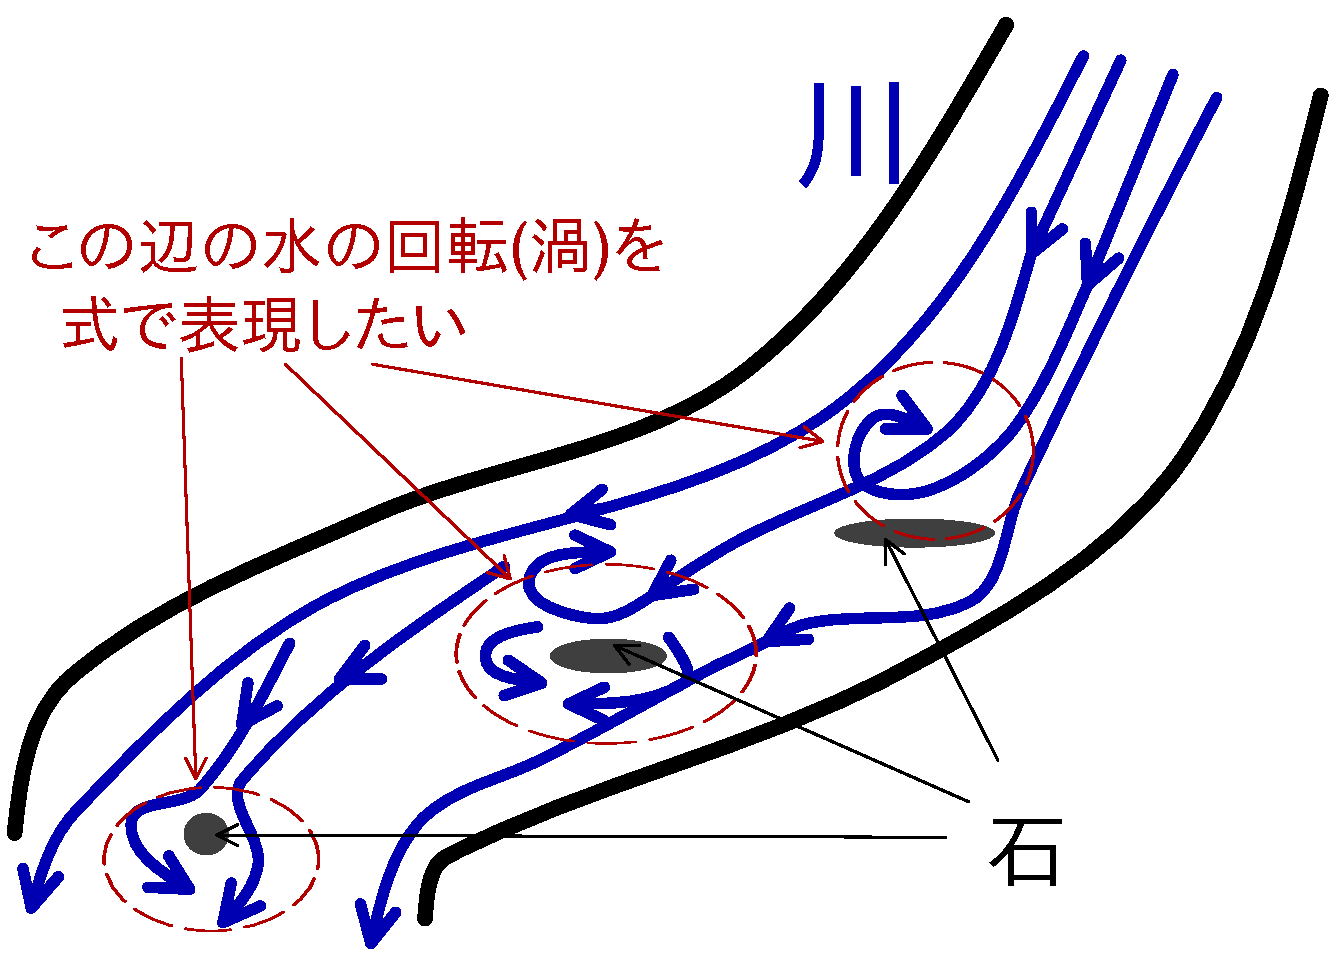
\includegraphics[keepaspectratio, width=4cm,height=2.87cm,clip]{image_rot_1.pdf}
                        \caption{川で生じる渦のイメージ}
                        \label{fig:image_rot_1}
                    \end{center}
                \end{figure}

        物体の回転を扱ったときは,直接的に物体そのものの運動を
        考えることができた.ところが,水などの流体は物体とは異なり,
        その流れ自体を物体と同じように考えるとややこしい.
        そこで,どのような流れかを知るために,川の上に
        葉を置いてみるのだ.葉は,水の流れに従って移動する.
        この葉の動きを観察することにより,
        川の様子を探ることができる.川の全体の
        様子を把握したい場合には,その川のいたるところに
        葉を置いて見て,その葉がどのような動きをするかを,
        観察すればよい.

        葉が1つの場所にとどまっていて,その場で
        回転している状況を想定する.この回転面に $x-y$ 面をとる
            \footnote{
                これは葉が置かれている表面,つまり水面に $x-y$ にとるのと同じである.
            }.
        そして,葉が回転している一点を原点にとる.
                \begin{figure}[hbt]
                    \begin{tabular}{cc}
                        \begin{minipage}{0.5\hsize}
                    \begin{center}
                        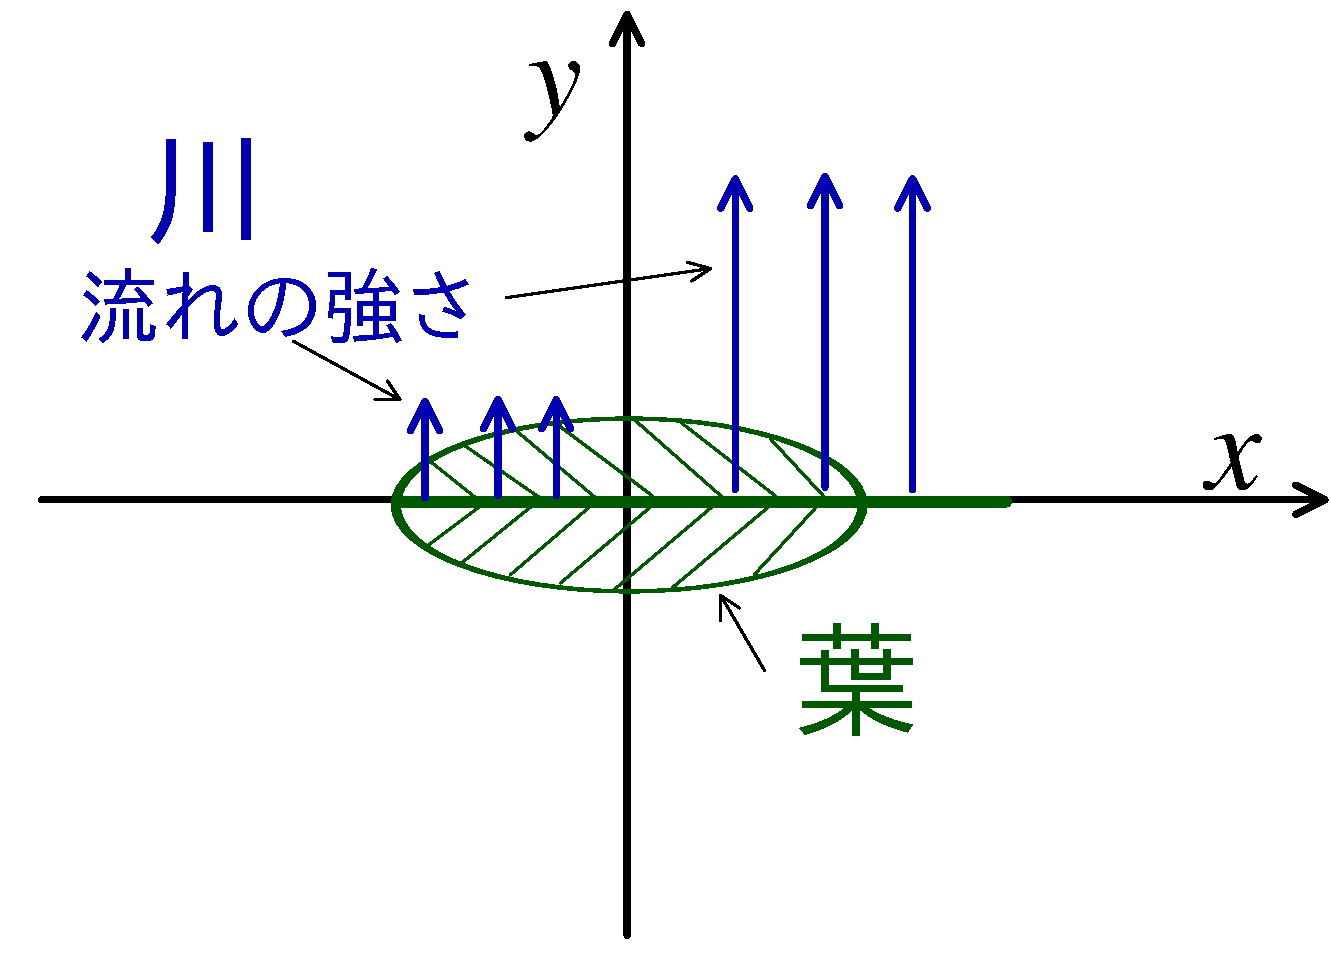
\includegraphics[keepaspectratio, width=4cm,height=2.87cm,clip]{rotrotrot.pdf}
                        \caption{回転(渦)が生じるための条件}
                        \label{fig:rotrotrot}
                    \end{center}
                        \end{minipage}
                        \begin{minipage}{0.5\hsize}
                    \begin{center}
                        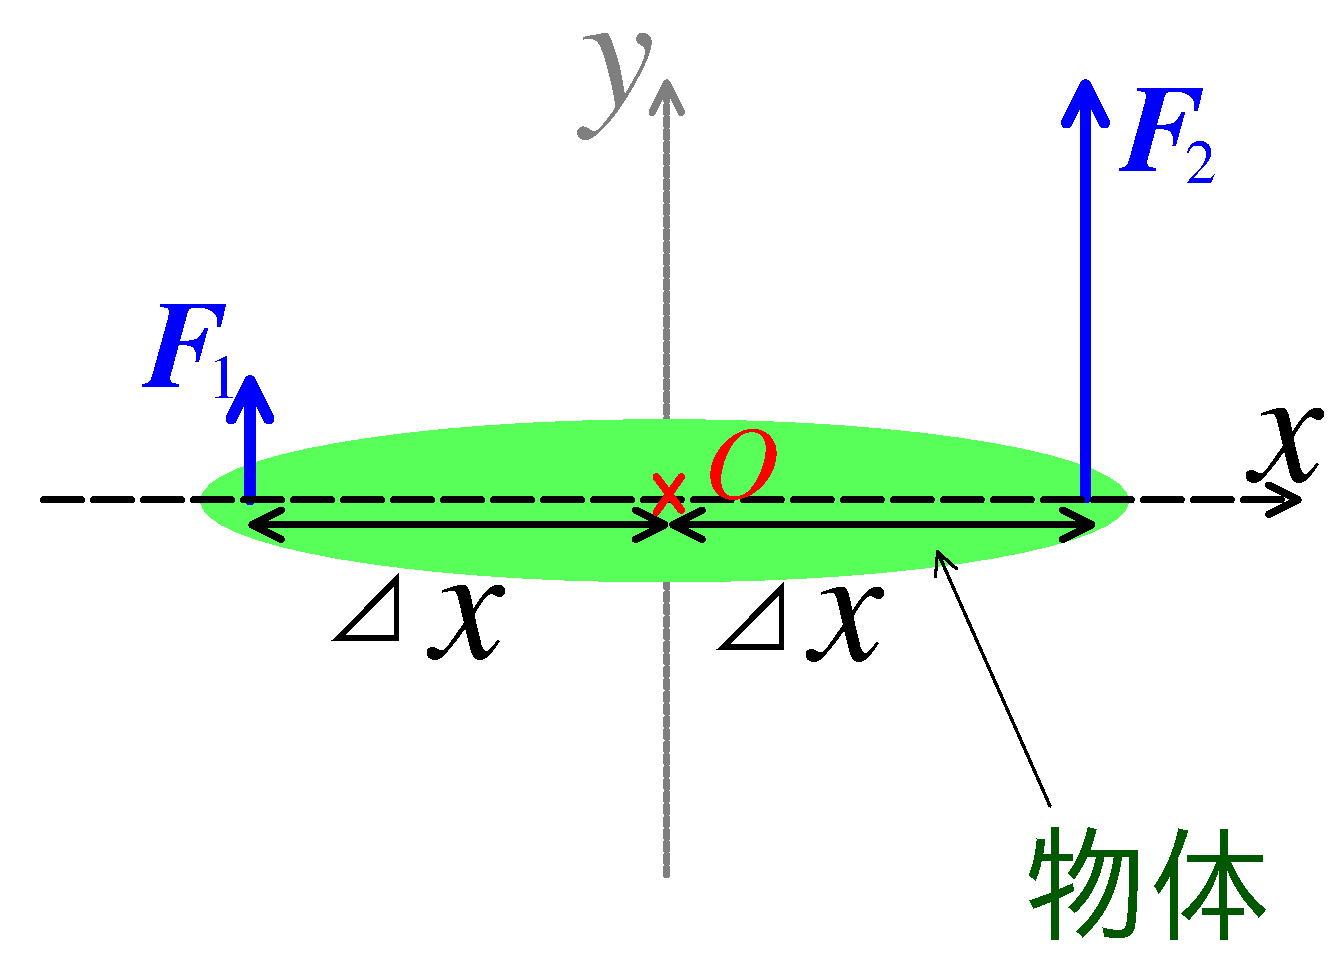
\includegraphics[keepaspectratio, width=4cm,height=2.87cm,clip]{rot_gaiseki1.pdf}
                        \caption{物体(葉)の回転1}
                        \label{fig:rot_gaiseki1}
                    \end{center}
                        \end{minipage}
                    \end{tabular}
                \end{figure}

        葉が原点を中心に回転するには,
        水の流れが原点の中心を境に,
        その勢いが異なっていればよい.
        図\ref{fig:rotrotrot}でいえば,左側の勢いと右側の勢いが
        違っていればよいということである.
        この図はもっと簡単になる.

        この図\ref{fig:rot_gaiseki1}で,左右両方の原点を中心とする力のモーメント
        を考えれば,左側が $F_{1}\Delta x$ であり,右側が $F_{2}\Delta x$ である.
        ここで,図より $F_{1}<F_{2}$ であるから($\Delta x$ は共通であるとする),
        この二つの力のモーメントのは互いに異なった値であり,従って,
        物体は回転をしているはずである
            \footnote{
                回転するように仮定を設けいているので,当たり前と言ってしまえばそうだが,
                確かに回転を表現できるという確認をここでしたのである.
            }.

        ここからが少しヤッカイな部分だが,それは今考えている対象は
        物体の回転ではなく水の回転,つまり“渦”である.
        この渦とはベクトルの回転である.
        物体の回転そのものを
        見るときは力のモーメントを考えればよかったが,
        ベクトルの回転では力のモーメントなんてものは直接には定義できない.
        だから,ベクトル(渦)の上に物体を置いて,その回転でもって
        ベクトルの回転の様子をうかがってみようとしたのである.
        そしてそれによって,ベクトルの回転の様子を,物体の回転として
        観測できることが分かった.この考えをもっと進めていこう.
        簡単のために,原点付近の水の様子を考えてみる.

        力の方向が左右で同じ方向を向いていなくともかまわない.
                \begin{figure}[hbt]
                    \begin{tabular}{cc}
                        \begin{minipage}{0.5\hsize}
                    \begin{center}
                        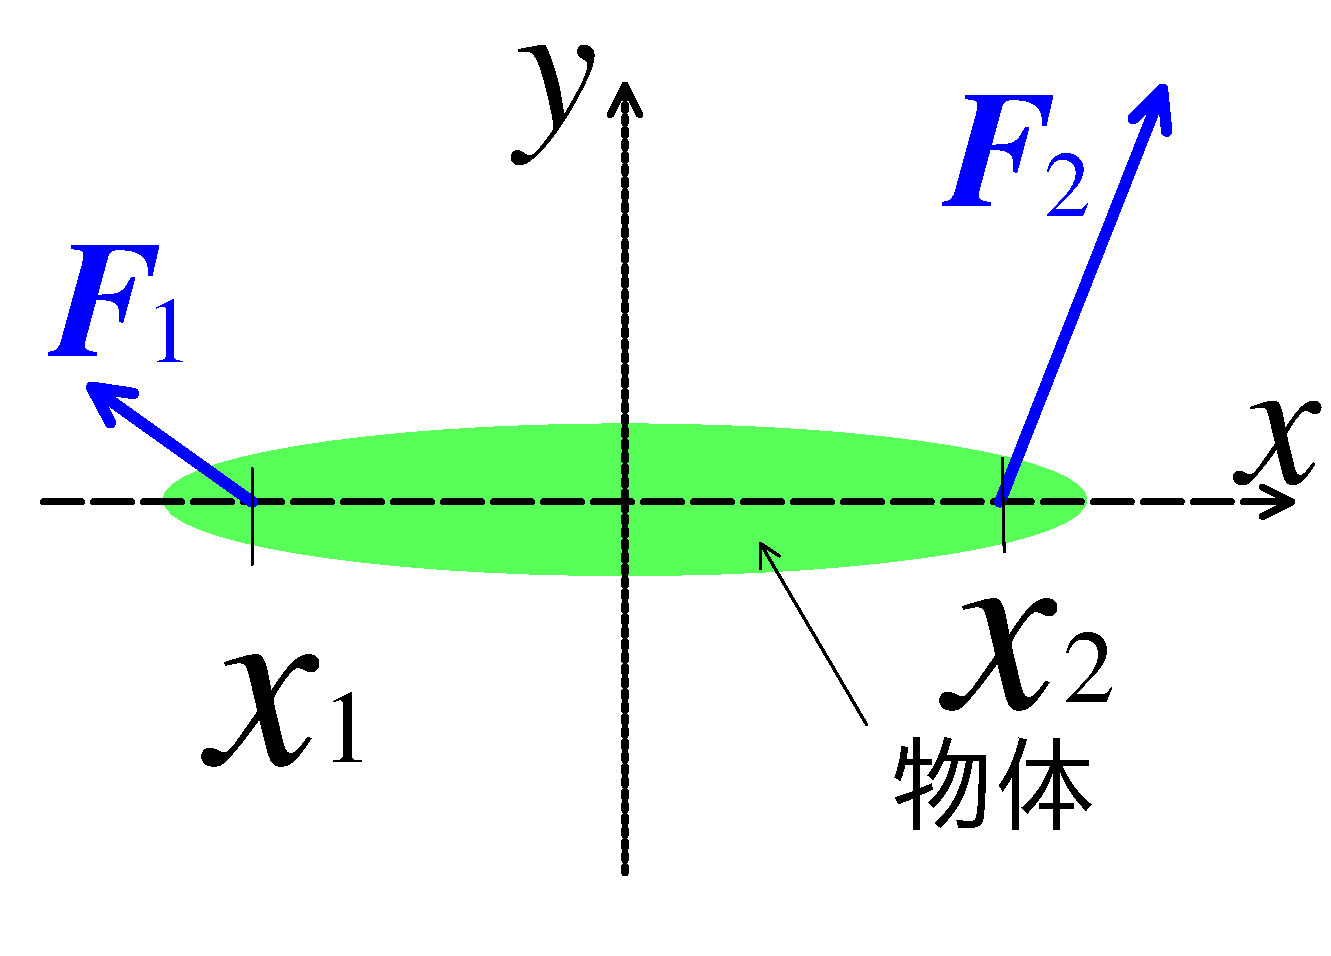
\includegraphics[keepaspectratio, width=4cm,height=2.87cm,clip]{rot_gaiseki2.pdf}
                        \caption{物体(葉)の回転2}
                        \label{fig:rot_gaiseki2}
                    \end{center}
                        \end{minipage}
                        \begin{minipage}{0.5\hsize}
                    \begin{center}
                        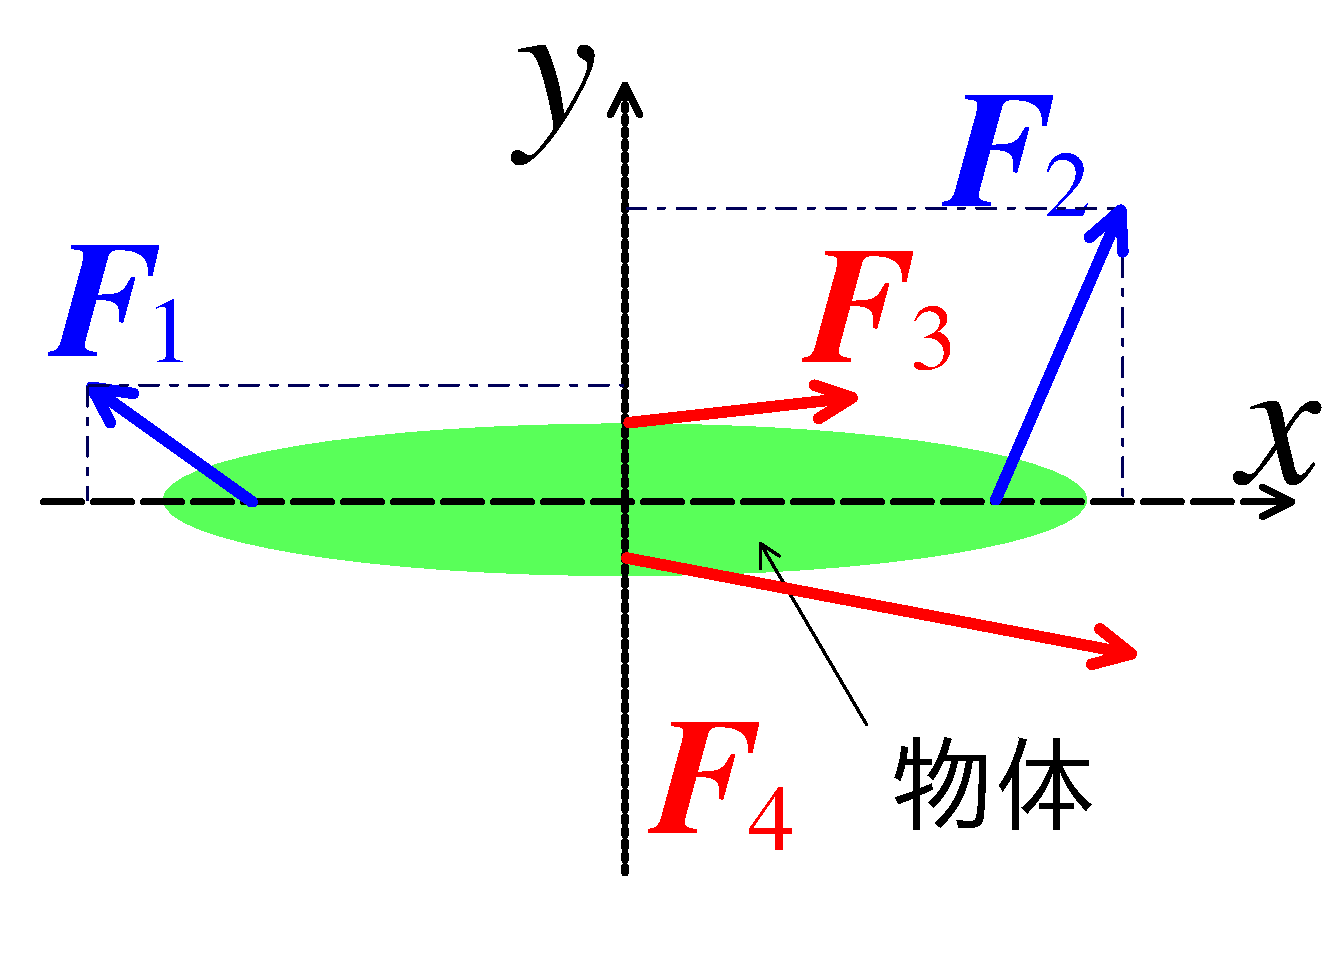
\includegraphics[keepaspectratio, width=4cm,height=2.87cm,clip]{rotation12.pdf}
                        \caption{物体(葉)の回転3}
                        \label{fig:rotation12}
                    \end{center}
                        \end{minipage}
                    \end{tabular}
                \end{figure}

        この図のような状況でベクトルの渦が起こるには,物体にかかる
        $x$ 方向と$y$ 方向の2方向で考えればよい.それを図\ref{fig:rotation12}に示す.

        ベクトル場とはここでは物体が水の流れから受ける力のことだが,
        これを $\bF(\,x,\,y\,)$ とする.
        ここでは話を簡単にするために,ベクトル場は時間に依存しないとした.

        先ほど考えた左右それぞれ力のモーメントの関係は $\bF_{1}\Delta x > \bF_{2}\Delta x$ であった.
        これを以下のように書き直す.
            \begin{align*}
                F_{1}\Delta x - F_{2}\Delta x &>& 0.  \\
                (F_{1} - F_{2})\Delta x &>& 0.
            \end{align*}
        さらにこの式の左辺は0より大きいので,
        何らかの定数,もしくは関数であるので,
        それを $a(\br\,,\,\,t)$ と
        書いて,
            \begin{equation*}
                (\bF_{1} - \bF_{2})\Delta x =a(\br\,,\,\,t)
            \end{equation*}
        とする.今考えている力 $F$ は,$x$ 座標と $y$ 座標ごとに違うはずである.
        つまり,$F$ は $x$ と $y$ の関数であるから,
            \begin{equation*}
                ( F(x_{1} ,\, y_{1}) - F(x_{2} ,\, y_{2}) )\Delta x =a(\br\,,\,\,t).
            \end{equation*}
        今考えているのは,原点付近の水の回転の様子であり,
        $x_{1}$ と $x_{2}$ はさほど離れていないと考えてよい.
        $x_{1}$ と $x_{2}$ の距離は前の図で $2\Delta x$ としていた.
        $2\Delta x$ を $h$ に置き換えてしまおう.
        つまり,$x_{2} = x_{1} + h$ である.
            \begin{equation*}
                ( F(x_{1} ,\, y_{1}) - F(x_{1} + h ,\, y_{2}) )\Delta x =a(\br\,,\,\,t).
            \end{equation*}
        上式の左辺第一項と第二項を入れ替えてみよう.
            \begin{equation*}
                ( F(x_{1} + h ,\, y_{2})  -  F(x_{1} ,\, y_{1})  )\Delta x = -a(\br\,,\,\,t).
            \end{equation*}

        ところで,物体の回転を現すには
        ベクトルの外積を用いた.

        ベクトル $\bA=(A_{x},\, A_{y},\, A_{z})$ の回転 $\drot$ は次式で定義される.
            \begin{align}
                \drot\bA:=
                \left(
                \frac{\rd A_{z}}{\rd y}-\frac{\rd A_{y}}{\rd z}\, ,\,\,
                \frac{\rd A_{x}}{\rd z}-\frac{\rd A_{z}}{\rd x}\, ,\,\,
                \frac{\rd A_{y}}{\rd x}-\frac{\rd A_{x}}{\rd y}
                \right)
            \end{align}

 \subsubsection{ベクトルの勾配($\rm{grad}$)}
        ベクトル $\bA=(A_{x},\, A_{y},\, A_{z})$ の勾配 $\dgrad$ は次式で定義される.
            \begin{align}
                \ddiv\bA:=
                \left(
                \frac{\rd \bA}{\rd x}\, ,\,\,
                \frac{\rd \bA}{\rd y}\, ,\,\,
                \frac{\rd \bA}{\rd z}
                \right)
            \end{align}




 \subsubsection{ベクトル解析の公式(演算子)}
            \begin{align}
                \Delta:=
                \mathrm{div\, grad}=
                \frac{\rd^{2}}{\rd x^{2}}+
                \frac{\rd^{2}}{\rd y^{2}}+
                \frac{\rd^{2}}{\rd z^{2}}
            \end{align}
            \begin{align}
                \mathrm{rot\, rot}
                =\mathrm{grad\, div}-\Delta
            \end{align}



 \subsubsection{ストークスの定理}
        任意の閉曲線を $l$,この閉曲線を縁とする曲面を $S_{l}$ と表す.
        また,閉曲線 $l$ の単位接線ベクトルを $\bt$ と表す.このとき,
        任意の3次元ベクトル $\bA$ に対して,
            \begin{align}
                \int_{S_{l}} (\drot \bA)\cdot\textit{\textbf{n}}\,\df S_{l}
                =\oint_{l} \bA\cdot\bt\,\df l
            \end{align}
        が成り立つ.これを \textbf{ストークスの定理} という.

